% 与英文单栏版保持相同物理尺寸，单元格字号 7.2 pt。
\begin{figure}[t]
\centering
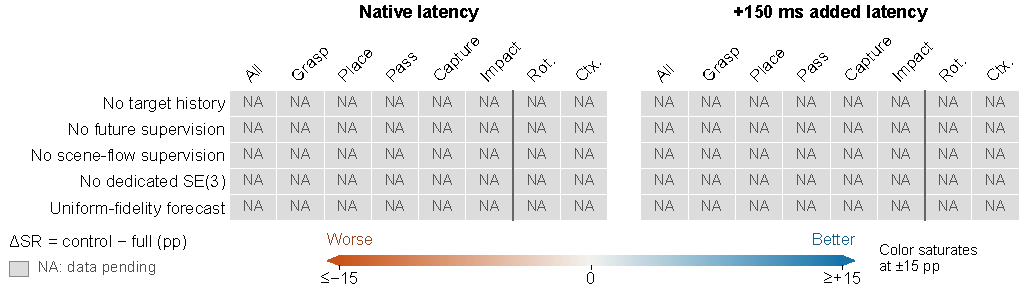
\includegraphics[width=3.25in]{Fig5/fig5.pdf}
\caption{\textbf{按任务的消融效应（设计预览；数据待齐）。}
$\Delta$SR = SR(对照) $-$ SR(完整模型)，单位为百分点；色阶在 $\pm$15 处饱和。
各对照定义见表~\ref{tab:design}。Rot./Ctx. 分别表示预先声明、可重叠的旋转敏感组和环境活跃组
（表~\appref{tab:roles}）。计划先对每个场景的三个训练种子取平均，再对各列内任务等权聚合，
保留 \texttt{t3\_phase}。将以粗体标出未作多重比较校正、且不含零的配对 95\% 场景自助法区间；
区间以给定训练权重为条件（附录~\appref{app:statistics}）。灰色 NA 表示尚无合格配对结果或估计。}
\label{fig:analysis}
\end{figure}
